% questions.tex —— 2009 年·普通高等学校招生考试·广东卷·理科 · 题目内容片段（无答案）
% 由 tools/generate_projects.py 依来源总账自 2009/2009_数学真题_广东理_试题.md 生成，勿手改（改源 MD 后重跑）


状态：needs-review；依固定候选 PDF 两页（印刷页 519–520）逐题核验，图形已矢量重绘。原页未印分值，不补。原页第 18 题第 (2) 问印作「直线 $FG_1\perp FEE_1$」，未印「平面」二字，照录原页并在解析中说明。原页二、填空题第 9—15 题连续排印，未印「13—15 为选做题（三选二）」的作答说明；本库按原页字面照录，13—15 三题均转录并各给答案（见 ISSUE-1501）。

\gkpart{一、选择题}

\Needspace{0.4\textheight}
\begingroup
\renewenvironment{question}{\Needspace{0.4\textheight}}{}
\begin{question}
\gkti{1}已知全集 $U=\mathbf R$，集合 $M=\{x\mid -2\leqslant x-1\leqslant 2\}$ 和 $N=\{x\mid x=2k-1,\ k=1,2,\cdots\}$ 的关系的韦恩（Venn）图如图所示，则阴影部分所示的集合的元素共有（　）

（A）$3$ 个

（B）$2$ 个

（C）$1$ 个

（D）无穷个
\nopagebreak[4]
\begin{center}% 2009 年广东卷（理科）第 1 题：全集 U 中集合 N、M 的韦恩图，阴影为 N∩M。
% 来源 PDF：.work/ocr-local/sources/2009广东理.pdf
% SHA-256：5256b35235a042e254d36c111af3eda0f5dd8f552664021d0bace5c05582ad04
% 原页：第 1 页（A3 四栏）第 1 栏，印刷页 519。
% 绘制依据：矩形表示 U，左圆 N、右圆 M 相交，交集透镜（N∩M）填灰；
%   原页只在矩形左上角标 U，两圆内分别标 N、M。
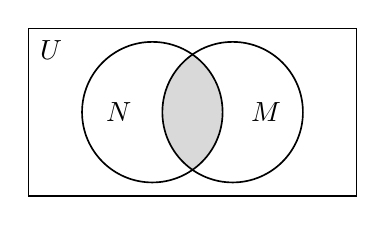
\begin{tikzpicture}[scale=0.85, semithick, every node/.style={inner sep=2pt}]
  \draw (0,0) rectangle (4.9,2.5);
  \node[anchor=north west] at (0.08,2.42) {$U$};
  \begin{scope}
    \clip (1.85,1.25) circle (1.05);
    \fill[gray!30] (3.05,1.25) circle (1.05);
  \end{scope}
  \draw (1.85,1.25) circle (1.05);
  \draw (3.05,1.25) circle (1.05);
  \node at (1.35,1.25) {$N$};
  \node at (3.55,1.25) {$M$};
\end{tikzpicture}
\end{center}
\nopagebreak[4]
\end{question}
\endgroup
\begin{question}
\gkti{2}设 $z$ 是复数，$\alpha(z)$ 表示满足 $z^n=1$ 的最小正整数 $n$，则对虚数单位 $\mathrm i$，$\alpha(\mathrm i)=$（　）

（A）$8$

（B）$6$

（C）$4$

（D）$2$

\end{question}
\begin{question}
\gkti{3}若函数 $y=f(x)$ 是函数 $y=a^x$（$a>0$，且 $a\neq1$）的反函数，其图象经过点 $(\sqrt a,a)$，则 $f(x)=$（　）

（A）$\log_2 x$

（B）$\log_{\frac12}x$

（C）$\frac{1}{2^x}$

（D）$x^2$

\end{question}
\begin{question}
\gkti{4}已知等比数列 $\{a_n\}$ 满足 $a_n>0$，$n=1,2,\cdots$，且 $a_5\cdot a_{2n-5}=2^{2n}$（$n\geqslant3$），则当 $n\geqslant1$ 时，$\log_2 a_1+\log_2 a_3+\cdots+\log_2 a_{2n-1}=$（　）

（A）$n(2n-1)$

（B）$(n+1)^2$

（C）$n^2$

（D）$(n-1)^2$

\end{question}
\begin{question}
\gkti{5}给定下列四个命题：

① 若一个平面内的两条直线与另一个平面都平行，那么这两个平面相互平行；

② 若一个平面经过另一个平面的垂线，那么这两个平面相互垂直；

③ 垂直于同一直线的两条直线相互平行；

④ 若两个平面垂直，那么一个平面内与它们的交线不垂直的直线与另一个平面也不垂直．

其中，为真命题的是（　）

（A）①和②

（B）②和③

（C）③和④

（D）②和④

\end{question}
\begin{question}
\gkti{6}一质点受到平面上的三个力 $\boldsymbol F_1$，$\boldsymbol F_2$，$\boldsymbol F_3$（单位：牛顿）的作用而处于平衡状态．已知 $\boldsymbol F_1$，$\boldsymbol F_2$ 成 $60^\circ$ 角，且 $\boldsymbol F_1$，$\boldsymbol F_2$ 的大小分别为 $2$ 和 $4$，则 $\boldsymbol F_3$ 的大小为（　）

（A）$6$

（B）$2$

（C）$2\sqrt5$

（D）$2\sqrt7$

\end{question}
\begin{question}
\gkti{7}2010 年广州亚运会组委会要从小张、小赵、小李、小罗、小王五名志愿者中选派四人分别从事翻译、导游、礼仪、司机四项不同工作，若其中小张和小赵只能从事前两项工作，其余三人均能从事这四项工作，则不同的选派方案共有（　）

（A）$36$ 种

（B）$12$ 种

（C）$18$ 种

（D）$48$ 种

\Needspace{0.4\textheight}
\end{question}
\begingroup
\renewenvironment{question}{\Needspace{0.4\textheight}}{}
\begin{question}
\gkti{8}已知甲、乙两车由同一起点同时出发，并沿同一路线（假定为直线）行驶．甲车、乙车的速度曲线分别为 $v_{\text{\text{甲}}}$ 和 $v_{\text{\text{乙}}}$（如图所示）．那么对于图中给定的 $t_0$ 和 $t_1$，下列判断中一定正确的是（　）

（A）在 $t_1$ 时刻，甲车在乙车前面

（B）$t_1$ 时刻后，甲车在乙车后面

（C）在 $t_0$ 时刻，两车的位置相同

（D）$t_0$ 时刻后，乙车在甲车前面
\nopagebreak[4]
\begin{center}% 2009 年广东卷（理科）第 8 题：甲、乙两车的速度—时间曲线。
% 来源 PDF：.work/ocr-local/sources/2009广东理.pdf
% SHA-256：5256b35235a042e254d36c111af3eda0f5dd8f552664021d0bace5c05582ad04
% 原页：第 1 页（A3 四栏）第 2 栏，印刷页 519。
% 绘制依据：v(t) 纵轴、t 横轴；v甲 自原点陡升后上凸（先快后慢），v乙 自原点平缓
%   后下凸（先慢后快），两线在 t0 之前相交；t0、t1 两处画竖直虚线至 v甲 曲线。
\begin{tikzpicture}[scale=1.0, semithick, every node/.style={inner sep=2pt}]
  \draw[->,>=stealth] (0,0) -- (5.6,0) node[below] {$t$};
  \draw[->,>=stealth] (0,0) -- (0,3.5) node[right] {$v(t)$};
  \node[below left] at (0,0) {$O$};

  % v甲：陡升后趋缓
  \draw[thick] (0,0) .. controls (0.55,1.35) and (1.5,2.05) .. (2.6,2.25)
    .. controls (3.4,2.4) and (4.1,2.6) .. (4.7,3.0);
  % v乙：平缓起步后急速上升
  \draw[thick] (0,0) .. controls (1.6,0.18) and (2.6,0.75) .. (3.35,1.75)
    .. controls (3.85,2.35) and (4.3,2.9) .. (4.6,3.35);

  \draw[dashed] (3.55,0) -- (3.55,2.44);
  \draw[dashed] (4.0,0) -- (4.0,2.56);
  \node[below] at (3.55,0) {$t_0$};
  \node[below] at (4.0,0) {$t_1$};

  \node at (1.95,2.55) {$v_{\text{甲}}$};
  \node at (1.75,0.8) {$v_{\text{乙}}$};
\end{tikzpicture}
\end{center}
\nopagebreak[4]
\end{question}
\endgroup
\gkpart{二、填空题}

\Needspace{0.4\textheight}
\begingroup
\renewenvironment{question}{\Needspace{0.5\textheight}}{}
\begin{question}
\gkti{9}随机抽取某产品 $n$ 件，测得其长度分别为 $a_1,a_2,\cdots,a_n$，则如图所示的程序框图输出的 $s=$\gkblank{}，$s$ 表示的样本的数字特征是\gkblank{}．（注：框图中的赋值符号“$=$”也可以写成“$\leftarrow$”或“$:=$”）
\nopagebreak[4]
\begin{center}% 2009 年广东卷（理科）第 9 题：求样本平均数 s 的程序框图。
% 来源 PDF：.work/ocr-local/sources/2009广东理.pdf
% SHA-256：5256b35235a042e254d36c111af3eda0f5dd8f552664021d0bace5c05582ad04
% 原页：第 1 页（A3 四栏）第 2 栏，印刷页 519。
% 绘制依据：开始 → 输入 n, a1, …, an → s=0, i=1 → 判断 i≤n：
%   是时 s←((i−1)×s+a_i)/i、i←i+1 后回环；否时输出 s、结束。
\begin{tikzpicture}[semithick, every node/.style={inner sep=3pt},
  box/.style={draw, minimum width=2.1cm, minimum height=0.55cm},
  io/.style={draw, trapezium, trapezium left angle=70, trapezium right angle=110,
             minimum width=2.9cm, minimum height=0.55cm},
  dec/.style={draw, diamond, aspect=2, inner sep=1pt,
              minimum width=2.3cm, minimum height=1.0cm}]

  \node[box, rounded corners=3pt] (start) at (0,0) {开始};
  \node[io] (input) at (0,-1.1) {输入 $n,a_1,a_2,\cdots,a_n$};
  \node[box] (init) at (0,-2.2) {$s=0,\ i=1$};
  \node[dec] (test) at (0,-3.6) {$i\leqslant n$?};
  \node[io] (out) at (0,-5.2) {输出 $s$};
  \node[box, rounded corners=3pt] (end) at (0,-6.3) {结束};

  \node[box] (assign) at (4.0,-3.6)
    {$s=\dfrac{(i-1)\times s+a_i}{i}$};
  \node[box] (inc) at (4.0,-2.6) {$i=i+1$};

  \draw[->,>=stealth] (start) -- (input);
  \draw[->,>=stealth] (input) -- (init);
  \draw[->,>=stealth] (init) -- (test);
  \draw[->,>=stealth] (test) -- node[left] {否} (out);
  \draw[->,>=stealth] (out) -- (end);
  \draw[->,>=stealth] (test.east) -- node[above] {是} (assign.west);
  \draw[->,>=stealth] (assign.north) -- (inc.south);
  \draw[->,>=stealth] (inc.west) -- (0,-2.6);
\end{tikzpicture}
\end{center}
\nopagebreak[4]
\end{question}
\endgroup
\begin{question}
\gkti{10}若平面向量 $\boldsymbol a$，$\boldsymbol b$ 满足 $|\boldsymbol a+\boldsymbol b|=1$，$\boldsymbol a+\boldsymbol b$ 平行于 $x$ 轴，$\boldsymbol b=(2,-1)$，则 $\boldsymbol a=$\gkblank{}。

\end{question}
\begin{question}
\gkti{11}已知椭圆 $G$ 的中心在坐标原点，长轴在 $x$ 轴上，离心率为 $\dfrac{\sqrt3}{2}$，且 $G$ 上一点到 $G$ 的两个焦点的距离之和为 $12$，则椭圆 $G$ 的方程为\gkblank{}。

\end{question}
\begin{question}
\gkti{12}已知离散型随机变量 $X$ 的分布列如下表．若 $EX=0$，$DX=1$，则 $a=$\gkblank{}，$b=$\gkblank{}。

\begin{center}
\begin{tabular}{ccccc}
\toprule
$X$ & $-1$ & $0$ & $1$ & $2$ \\
\midrule
$P$ & $a$ & $b$ & $c$ & $\dfrac{1}{12}$ \\
\bottomrule
\end{tabular}
\end{center}

\end{question}
\begin{question}
\gkti{13}若直线 $l_1:\begin{cases}x=1-2t,\\ y=2+kt,\end{cases}$（$t$ 为参数）与直线 $l_2:\begin{cases}x=s,\\ y=1-2s,\end{cases}$（$s$ 为参数）垂直，则 $k=$\gkblank{}。

\end{question}
\begin{question}
\gkti{14}不等式 $\dfrac{|x+1|}{|x+2|}\geqslant1$ 的实数解为\gkblank{}。

\Needspace{0.4\textheight}
\end{question}
\begingroup
\renewenvironment{question}{\Needspace{0.4\textheight}}{}
\begin{question}
\gkti{15}如图，点 $A$，$B$，$C$ 是圆 $O$ 上的点，且 $AB=4$，$\angle ACB=45^\circ$，则圆 $O$ 的面积等于\gkblank{}。
\nopagebreak[4]
\begin{center}% 2009 年广东卷（理科）第 15 题：圆 O 上三点 A、B、C，AB=4，∠ACB=45°。
% 来源 PDF：.work/ocr-local/sources/2009广东理.pdf
% SHA-256：5256b35235a042e254d36c111af3eda0f5dd8f552664021d0bace5c05582ad04
% 原页：第 1 页（A3 四栏）第 3 栏，印刷页 519。
% 绘制依据：AB 为竖直弦（B 在右上、A 在右下），C 在下方，连 CA、CB；
%   圆周角 ∠ACB=45° 对应 AB 所对圆心角 90°。
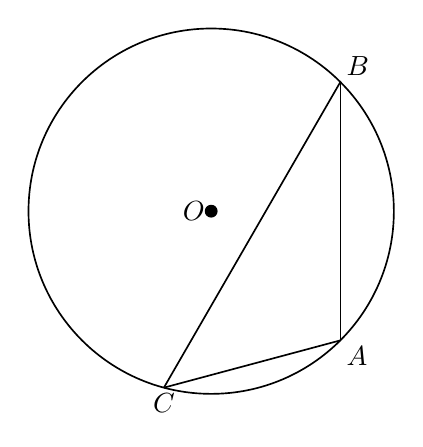
\begin{tikzpicture}[scale=1.45, semithick, every node/.style={inner sep=2pt}]
  \draw (0,0) circle (1.6);
  \coordinate (O) at (0,0);
  \coordinate (B) at (45:1.6);
  \coordinate (A) at (-45:1.6);
  \coordinate (C) at (255:1.6);

  \draw (A) -- (B);
  \draw (C) -- (B);
  \draw (C) -- (A);

  \fill (O) circle (1.6pt);
  \node[left] at (0,0) {$O$};
  \node[above right] at (B) {$B$};
  \node[below right] at (A) {$A$};
  \node[below] at (C) {$C$};
\end{tikzpicture}
\end{center}
\nopagebreak[4]
\end{question}
\endgroup
\gkpart{三、解答题}

\begin{question}
\gkti{16}已知向量 $\boldsymbol a=(\sin\theta,-2)$ 与 $\boldsymbol b=(1,\cos\theta)$ 互相垂直，其中 $\theta\in\left(0,\dfrac{\pi}{2}\right)$．

（1）求 $\sin\theta\cos\theta$ 的值；

（2）若 $\sin(\theta-\varphi)=\dfrac{\sqrt{10}}{10}$，$0<\varphi<\dfrac{\pi}{2}$，求 $\cos\varphi$ 的值．

\Needspace{0.4\textheight}
\end{question}
\begingroup
\renewenvironment{question}{\Needspace{0.5\textheight}}{}
\begin{question}
\gkti{17}根据空气质量指数 API（为整数）的不同，可将空气质量分级如下表：对某城市一年（365 天）的空气质量进行监测，获得 API 数据按照区间 $[0,50]$，$(50,100]$，$(100,150]$，$(150,200]$，$(200,250]$，$(250,300]$ 进行分组，得到频率分布直方图如图．

\begin{center}
\begingroup\setlength{\tabcolsep}{4pt}
\begin{tabular}{ccccclll}
\toprule
API & 0～50 & 51～100 & 101～150 & 151～200 & 201～250 & 251～300 & $>300$ \\
\midrule
级别 & I & II & III$_1$ & III$_2$ & IV$_1$ & IV$_2$ & V \\
状况 & 优 & 良 & 轻微污染 & 轻度污染 & 中度污染 & 中重度污染 & 重度污染 \\
\bottomrule
\end{tabular}
\endgroup
\end{center}

（1）求直方图中 $x$ 的值；

（2）计算一年中空气质量分别为良和轻微污染的天数；

（3）求该城市某一周至少有 2 天的空气质量为良或轻微污染的概率．

（结果用分数表示．已知 $5^7=78125$，$2^7=128$，$\dfrac{3}{1825}+\dfrac{2}{365}+\dfrac{7}{1825}+\dfrac{3}{1825}+\dfrac{8}{9125}=\dfrac{123}{9125}$，$365=73\times5$）
\nopagebreak[4]
\begin{center}% 2009 年广东卷（理科）第 17 题：空气质量指数 API 的频率分布直方图。
% 来源 PDF：.work/ocr-local/sources/2009广东理.pdf
% SHA-256：5256b35235a042e254d36c111af3eda0f5dd8f552664021d0bace5c05582ad04
% 原页：第 1 页（A3 四栏）第 4 栏，印刷页 519。
% 绘制依据：组距 50，六组 [0,50]、[50,100]、[100,150]、[150,200]、[200,250]、
%   [250,300]；纵轴为「频率/组距」，各柱高依次为 3/1825、x、2/365、7/1825、
%   3/1825、8/9125（以 1/9125 为单位取 15、59.5、50、35、15、8，与原页比例一致）。
\begin{tikzpicture}[x=0.040cm, y=0.070cm, semithick,
  every node/.style={inner sep=2pt}]

  % 坐标轴
  \draw[->,>=stealth] (0,0) -- (345,0);
  \draw[->,>=stealth] (0,0) -- (0,84);
  \node[below right] at (345,0) {API};
  \node[anchor=west] at (12,76) {频率};
  \draw (12,72.5) -- (34,72.5);
  \node[anchor=west] at (12,69) {组距};

  % 六个柱
  \draw (0,0) rectangle (50,15);
  \draw (50,0) rectangle (100,59.5);
  \draw (100,0) rectangle (150,50);
  \draw (150,0) rectangle (200,35);
  \draw (200,0) rectangle (250,15);
  \draw (250,0) rectangle (300,8);

  % 虚线导引
  \draw[dashed] (0,59.5) -- (50,59.5);
  \draw[dashed] (0,50) -- (100,50);
  \draw[dashed] (0,35) -- (150,35);
  \draw[dashed] (50,15) -- (200,15);
  \draw[dashed] (0,8) -- (250,8);

  % 纵轴刻度值
  \node[left] at (0,59.5) {$x$};
  \node[left] at (0,50) {$\dfrac{2}{365}$};
  \node[left] at (0,35) {$\dfrac{7}{1825}$};
  \node[left, yshift=5pt] at (0,15) {$\dfrac{3}{1825}$};
  \node[left, yshift=-7pt] at (0,8) {$\dfrac{8}{9125}$};

  % 横轴刻度
  \node[below left] at (0,0) {$0$};
  \foreach \x in {50,100,150,200,250,300}
    \node[below] at (\x,0) {$\x$};
\end{tikzpicture}
\end{center}
\nopagebreak[4]
\Needspace{0.4\textheight}
\end{question}
\endgroup
\begingroup
\renewenvironment{question}{\Needspace{0.5\textheight}}{}
\begin{question}
\gkti{18}如图，已知正方体 $ABCD-A_1B_1C_1D_1$ 的棱长为 $2$，点 $E$ 是正方形 $BCC_1B_1$ 的中心，点 $F$、$G$ 分别是棱 $C_1D_1$、$AA_1$ 的中点．设点 $E_1$，$G_1$ 分别是点 $E$、$G$ 在平面 $DCC_1D_1$ 内的正投影．

（1）求以 $E$ 为顶点，以四边形 $FGAE$ 在平面 $DCC_1D_1$ 内的正投影为底面边界的棱锥的体积；

（2）证明：直线 $FG_1\perp FEE_1$；

（3）求异面直线 $E_1G_1$ 与 $EA$ 所成角的正弦值．
\nopagebreak[4]
\begin{center}% 2009 年广东卷（理科）第 18 题：棱长为 2 的正方体及其中的点 E、F、G。
% 来源 PDF：.work/ocr-local/sources/2009广东理.pdf
% SHA-256：5256b35235a042e254d36c111af3eda0f5dd8f552664021d0bace5c05582ad04
% 原页：第 2 页（A3 三栏）第 1 栏，印刷页 520。
% 绘制依据：斜二测式画法，前表面 A B B1 A1，纵深方向朝右上；D、C、D1、C1 为后表面
%   顶点。E 为正方形 BCC1B1 的中心，F 为 C1D1 中点，G 为 AA1 中点；E1、G1 分别是
%   E、G 在平面 DCC1D1 内的正投影（即 CC1、DD1 的中点）。
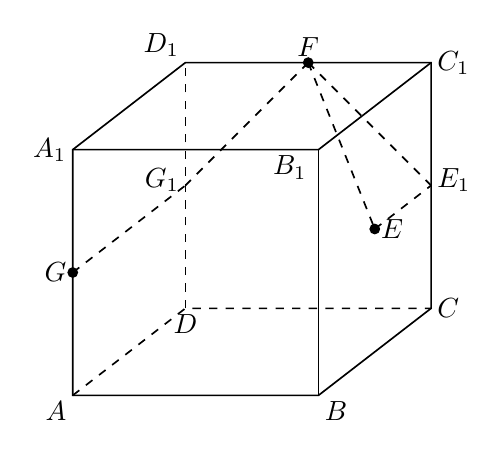
\begin{tikzpicture}[scale=1.3, semithick, every node/.style={inner sep=2pt}]

  \coordinate (A)  at (0,0);
  \coordinate (B)  at (2.4,0);
  \coordinate (A1) at (0,2.4);
  \coordinate (B1) at (2.4,2.4);
  \coordinate (D)  at (1.1,0.85);
  \coordinate (C)  at (3.5,0.85);
  \coordinate (D1) at (1.1,3.25);
  \coordinate (C1) at (3.5,3.25);
  \coordinate (E)  at (2.95,1.625);
  \coordinate (F)  at (2.3,3.25);
  \coordinate (G)  at (0,1.2);
  \coordinate (E1) at (3.5,2.05);
  \coordinate (G1) at (1.1,2.05);

  % 可见棱
  \draw (A) -- (B) -- (C) -- (C1) -- (D1) -- (A1) -- cycle;
  \draw (A1) -- (B1) -- (C1);
  \draw (B) -- (B1);

  % 不可见棱
  \draw[dashed] (A) -- (D) -- (C);
  \draw[dashed] (D) -- (D1);

  % 辅助线
  \draw[dashed] (F) -- (E);
  \draw[dashed] (F) -- (E1);
  \draw[dashed] (F) -- (G1);
  \draw[dashed] (E) -- (E1);
  \draw[dashed] (G) -- (G1);

  \fill (E) circle (1.5pt);
  \fill (F) circle (1.5pt);
  \fill (G) circle (1.5pt);

  \node[below left]  at (A)  {$A$};
  \node[below right] at (B)  {$B$};
  \node[right]       at (C)  {$C$};
  \node[below]       at (D)  {$D$};
  \node[left]        at (A1) {$A_1$};
  \node[below left, xshift=-2pt] at (B1) {$B_1$};
  \node[right]       at (C1) {$C_1$};
  \node[above left]  at (D1) {$D_1$};
  \node[right]       at (E)  {$E$};
  \node[above]       at (F)  {$F$};
  \node[left]        at (G)  {$G$};
  \node[right, yshift=2pt]  at (E1) {$E_1$};
  \node[left, yshift=2pt]   at (G1) {$G_1$};
\end{tikzpicture}
\end{center}
\nopagebreak[4]
\end{question}
\endgroup
\begin{question}
\gkti{19}已知曲线 $C:y=x^2$ 与直线 $l:x-y+2=0$ 交于两点 $A(x_A,y_A)$ 和 $B(x_B,y_B)$，且 $x_A<x_B$．记曲线 $C$ 在点 $A$ 和点 $B$ 之间那一段 $L$ 与线段 $AB$ 所围成的平面区域（含边界）为 $D$．设点 $P(s,t)$ 是 $L$ 上的任一点，且点 $P$ 与点 $A$ 和点 $B$ 均不重合．

（1）若点 $Q$ 是线段 $AB$ 的中点，试求线段 $PQ$ 的中点 $M$ 的轨迹方程；

（2）若曲线 $G:x^2-2ax+y^2-4y+a^2+\dfrac{51}{25}=0$ 与 $D$ 有公共点，试求 $a$ 的最小值．

\end{question}
\begin{question}
\gkti{20}已知二次函数 $y=g(x)$ 的导函数的图象与直线 $y=2x$ 平行，且 $y=g(x)$ 在 $x=-1$ 处取得极小值 $m-1$（$m\neq0$）．设 $f(x)=\dfrac{g(x)}{x}$．

（1）若曲线 $y=f(x)$ 上的点 $P$ 到点 $Q(0,2)$ 的距离的最小值为 $\sqrt2$，求 $m$ 的值；

（2）$k$（$k\in\mathbf R$）如何取值时，函数 $y=f(x)-kx$ 存在零点，并求出零点．

\end{question}
\begin{question}
\gkti{21}已知曲线 $C_n:x^2-2nx+y^2=0$（$n=1,2,\cdots$）．从点 $P(-1,0)$ 向曲线 $C_n$ 引斜率为 $k_n$（$k_n>0$）的切线 $l_n$，切点为 $P_n(x_n,y_n)$．

（1）求数列 $\{x_n\}$ 与 $\{y_n\}$ 的通项公式；

（2）证明：$x_1\cdot x_3\cdot x_5\cdots x_{2n-1}<\sqrt{\dfrac{1-x_n}{1+x_n}}<\sqrt2\sin\dfrac{x_n}{y_n}$．

\end{question}